\documentclass[10pt,twocolumn]{article}

% use the oxycomps style file
\usepackage{oxycomps}
\usepackage{multirow}
\usepackage{graphicx}

% usage: \fixme[comments describing issue]{text to be fixed}
% define \fixme as not doing anything special
\newcommand{\fixme}[2][]{#2}
% overwrite it so it shows up as red
\renewcommand{\fixme}[2][]{\textcolor{red}{#2}}
% overwrite it again so related text shows as footnotes
%\renewcommand{\fixme}[2][]{\textcolor{red}{#2\footnote{#1}}}

% read references.bib for the bibtex data
\bibliography{references}

% include metadata in the generated pdf file
\pdfinfo{
    /Title (The Occidental Computer Science Comprehensive Project: Goals, Timeline, Format, and Advice)
    /Author (Karlo Papa)
}

% set the title and author information
\title{Optimizing LSTM Models for Stock Price Prediction Within a Selected Portfolio}
\author{Karlo Papa}
\affiliation{Occidental College}
\email{kpapa@oxy.edu}

\begin{document}

\maketitle

\section{Introduction and Problem Context}
The Charles R. Blyth Fund, a six-figure student-run investment club at Occidental College, currently relies primarily on a six-month qualitative analysis timeline to guide its stock selection and asset allocation decisions. Although deep domain knowledge and qualitative research are invaluable, this approach consumes a lot of time and does not enable the fund to manage risk and asset allocation on a daily basis. To address these limitations, this project aims to develop quantitative machine learning (ML) methods that outperform baseline methods to allow the fund to manage day-to-day asset allocation and strengthen their 6-month investment research.

As financial markets increasingly adopt data-driven quantitative approaches, machine learning (ML)-based stock price forecasting has garnered significant interest from both the computer science and investment communities. These disciplines collaborate to address the complexities of non-stationary time series data, aiming to improve capital allocation and achieve superior investment performance. Gu, Kelly, and Xiu (2020) demonstrate that ML techniques, particularly neural networks, significantly enhance predictive accuracy in asset pricing by capturing complex, nonlinear interactions among predictors, leading to improved forecasts of asset returns \cite{Gu2020EmpiricalAssetPricing}. To remain competitive in this rapidly evolving landscape, the Blyth Fund must continue to evolve by equipping its emerging professional students with data literacy and technical competencies through integrating ML methodologies into its investment strategies.

Integrating machine learning (ML) in finance involves critically assessing ethical issues such as algorithmic bias, transparency, and accountability, alongside economic impacts like market stability and the democratization of investment opportunities. Kurshan et al. (2021) highlight the ethical and practical challenges in deploying AI and ML solutions within financial services, emphasizing issues such as ensuring fairness, mitigating bias, enhancing transparency, and addressing risks like market manipulation and systemic instability, all while balancing innovation with regulatory compliance \cite{Kurshan2021FairEthicalAI}. By leveraging ML methodologies, smaller investors like the Blyth Fund can implement sophisticated strategies traditionally reserved for larger firms, leveling the playing field and empowering a more diverse range of market participants. Addressing these ethical and societal considerations ensures that ML adoption is not only effective but also socially responsible, fostering stakeholder trust and contributing positively to the broader economic ecosystem.

This project optimizes Long Short-Term Memory (LSTM) models to effectively capture temporal dependencies in financial time-series data, advancing both academic research and practical financial applications. By providing smaller investment funds like the Blyth Fund with advanced predictive tools, the project enables more accurate and timely asset allocation decisions typically reserved for larger firms. The complexity of this endeavor arises from managing the non-stationary nature and inherent noise of financial data. By addressing these challenges, the project aims to enhance the fund’s investment strategies and deepen the understanding of machine learning applications in finance.

\section{Technical Background}

This section outlines key financial indicators and machine learning (ML) techniques for time-series forecasting used in this project.

\subsection{Terminology and Financial Indicators}

Stock prices are volatile and sequential, making them ideal for time-series analysis, which involves data points collected at uniform intervals. Figure \ref{fig:stock_i_close_price} shows the closing price of Stock I from 2020 to 2024, illustrating the sequential nature and inherent volatility of financial data.

\begin{figure}[htbp]
    \centering
    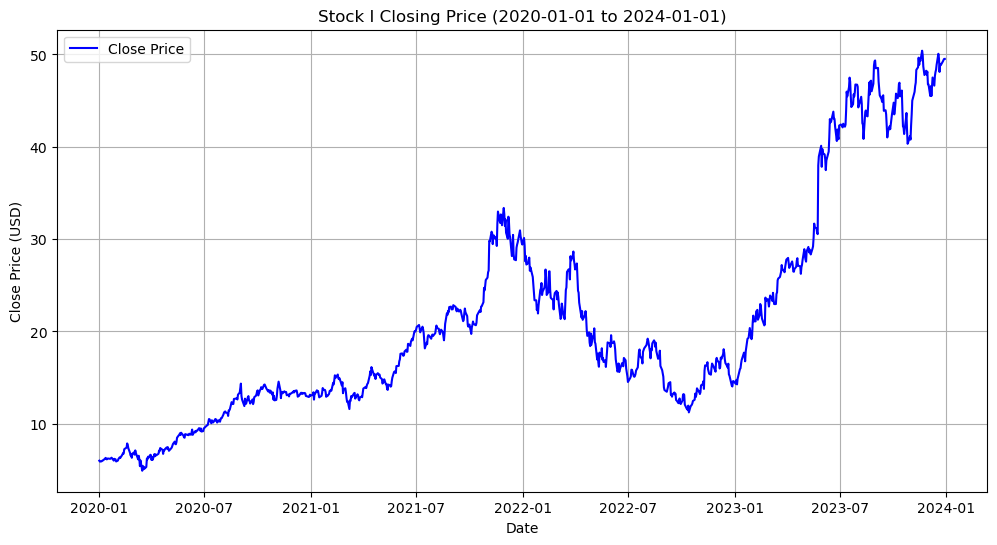
\includegraphics[width=\linewidth]{Stock_I_Close_Price.png}
    \caption{Stock I Closing Price (2020-01-01 to 2024-01-01). The sequential nature and volatility of stock prices are evident, emphasizing the importance of time-series forecasting techniques.}
    \label{fig:stock_i_close_price}
\end{figure}

\textit{Open, High, Low, and Close Prices:}  
\begin{itemize}
    \item \textit{Open Price:} The price at which a stock starts trading when the market opens for a specific period.
    \item \textit{High Price:} The highest price a stock reaches during the trading period.
    \item \textit{Low Price:} The lowest price a stock falls to during the trading period.
    \item \textit{Close Price:} The final price at which the stock is traded when the market closes.
\end{itemize}

\textit{Bollinger Bands (BB):}  
Bollinger Bands are volatility indicators calculated using a stock's SMA and standard deviations:
\[
\text{BB Upper} = \text{SMA} + 2 \cdot \sigma, \quad \text{BB Lower} = \text{SMA} - 2 \cdot \sigma
\]
where \(\sigma\) is the standard deviation. Bollinger Bands measure price fluctuations and help identify overbought or oversold conditions.

\textit{Volatility:}  
Volatility measures the degree of variation in a stock's price over time, often represented as the standard deviation of returns. Higher volatility indicates larger price swings, reflecting greater uncertainty.

\subsection{Simple and Exponential Moving Averages}
\textit{Simple Moving Average (SMA):}  
SMA averages a stock's closing prices over a set period, smoothing short-term fluctuations and highlighting trends:
\[
\text{SMA} = \frac{P_1 + P_2 + \dots + P_n}{n}
\]

\textit{Exponential Moving Average (EMA):}  
EMA gives more weight to recent data, making it more responsive to trends:
\[
\text{EMA}_t = P_t \times k + \text{EMA}_{t-1} \times (1 - k), \quad k = \frac{2}{N+1}
\]

\subsection{Classical Statistical Models}

Linear regression fits a line to minimize the error between predicted and actual values. It serves as a baseline for comparing advanced models \cite{James2021IntroStatLearning}.

\subsection{Advanced Neural Network Architectures}

Long Short-Term Memory (LSTM) networks, a type of recurrent neural network, handle long-range dependencies via gates that control information flow. This enables them to capture complex patterns in sequential data \cite{Hochreiter1997LSTM, Fischer2017LSTMFinance}.

\subsection{Sliding Window Approach}

The sliding window approach (size = 5, step = 2) structures data for training, validation, and testing. Within each window, the model uses pairs of sequential data points to predict the next value, iteratively sliding the window over the dataset to capture temporal dependencies. The window size determines the range of data included in each step, while the step size controls how far the window moves after each iteration \cite{Zhan2024SlidingWindow}. A portion of the window data is reserved for training, a smaller portion for validation during model training, and the value following the window is used for testing.

\textit{Example:} Consider a simplified dataset with sequential daily stock prices:

\[
\text{Dataset: } [1, 2, 3, 4, 5, 6, 7, 8, 9, 10]
\]

\begin{itemize}
    \item Window Size: 5
    \item Step Size: 2
    \item Training Ratio: 90\%
\end{itemize}

Using this approach, the data is processed as follows:

\begin{table}[h]
    \centering
    \caption{Sliding Window Example}
    \label{tab:sliding_window_example}
    \begin{tabular}{|c|l|}
        \hline
        \textbf{Window \#} & \textbf{Data} \\
        \hline
        1 & Training: {[1, 2] → 3, [2, 3] → 4} \\
          & Validation: {[3, 4] → 5} \\
          & Test: {[4, 5] → 6} \\
        \hline
        2 & Training: {[3, 4] → 5, [4, 5] → 6} \\
          & Validation: {[5, 6] → 7} \\
          & Test: {[6, 7] → 8} \\
        \hline
        3 & Training: {[5, 6] → 7, [6, 7] → 8} \\
          & Validation: {[7, 8] → 9} \\
          & Test: {[8, 9] → 10} \\
        \hline
    \end{tabular}
\end{table}

\subsection{Normalization and Training Optimization Techniques}

To enhance performance and address challenges in sequential data, the following techniques were employed:

\textit{Normalization with Robust Scaler:}  
The Robust Scaler normalizes data using the median and interquartile range (IQR), reducing outlier influence\cite{Passalis2021RobustNormalization}:
\[
z = \frac{X - \text{Median}}{\text{IQR}}
\]

\textit{Warm-Starting LSTM Models:}  
The LSTM is initialized with previously trained weights to retain learned patterns, reducing training time and improving convergence \cite{Ash2019WarmStarting}.

\textit{Early Stopping:}  
Training halts if validation loss does not improve over a set number of epochs, preventing overfitting and saving computation.

\textit{Model Evaluation and Weight Saving:}  
After training on each window, performance is evaluated using MAPE. Trained weights are saved for subsequent iterations, and predictions are made on the last sample of each window.

\subsection{Evaluation Metrics}

Mean Absolute Percentage Error (MAPE) measures prediction accuracy as a percentage:
\[
\text{MAPE} = \frac{100\%}{N} \sum_{t=1}^{N} \left| \frac{A_t - F_t}{A_t} \right|
\]

MAPE was chosen for its simplicity and ability to provide intuitive percentage-based error comparisons, aligning with the project’s focus on relative prediction accuracy.

\section{Prior Work}

Machine learning (ML) techniques have been increasingly applied to stock price prediction, driven by their ability to model complex relationships and dynamics in financial markets. This section reviews prior work across foundational financial modeling, advanced machine learning techniques, adaptive training strategies, and ethical considerations, highlighting their relevance and influence on this project.

\subsection{Foundations in Financial Modeling}

Traditional financial analysis relies on indicators such as moving averages to identify trends and generate trading signals. Bodie et al. \cite{Bodie2014Essentials} provide a foundational exploration of investment strategies and market behavior, establishing the groundwork for understanding how financial metrics like Simple Moving Average (SMA) and Exponential Moving Average (EMA) contribute to decision-making. However, while effective in stable environments, these heuristic tools often fail to adapt to rapid market changes.

Linear regression, a statistical technique extensively discussed by James et al. \cite{James2021IntroStatLearning}, has been employed as a baseline for financial forecasting. It provides a data-driven approach to uncover relationships between variables. While its simplicity makes it valuable for initial analysis, its assumption of linearity limits its ability to capture the complex, nonlinear relationships prevalent in financial markets.

\subsection{Advanced Machine Learning Techniques}

The advent of machine learning has revolutionized financial forecasting by enabling models to capture complex temporal dependencies and patterns. Recurrent Neural Networks (RNNs), particularly Long Short-Term Memory (LSTM) networks, have emerged as a key tool for sequential data analysis. Hochreiter and Schmidhuber \cite{Hochreiter1997LSTM} introduced LSTMs to address the vanishing gradient problem in standard RNNs, enabling these models to retain long-term dependencies effectively.

Fischer and Krauss \cite{Fischer2017LSTMFinance} applied LSTM networks to financial market predictions, demonstrating their superiority over traditional statistical methods in capturing intricate temporal dynamics in stock prices. Similarly, Malhotra et al. \cite{Malhotra2015LSTMAnomaly} showcased the versatility of LSTMs in detecting anomalies in time series data, further validating their robustness for financial applications. These studies underscore the potential of LSTM networks to model the nonlinear and time-dependent nature of financial data effectively.

\subsection{Adaptive Training Strategies}

Financial markets are inherently dynamic, necessitating adaptive approaches to training machine learning models. Zhan and Kim \cite{Zhan2024SlidingWindow} employed sliding window techniques to structure financial time series data, enabling models to incorporate the most recent data while capturing temporal dependencies. This approach ensures that models remain relevant as market conditions evolve and adapt to changing patterns. The concept of warm-starting, which leverages previously learned model weights during retraining, complements rolling window strategies and reduces the risk of overfitting by retaining prior knowledge while adapting to new patterns \cite{Ash2019WarmStarting}.

\subsection{Data Normalization and Preprocessing}

Preprocessing plays a crucial role in enhancing the performance of machine learning models in finance. Passalis et al. \cite{Passalis2021RobustNormalization} introduced a robust deep adaptive normalization framework that dynamically adjusts scaling parameters to reflect evolving data distributions. This approach ensures consistent model performance by mitigating the influence of outliers and adapting to non-stationary financial data. These preprocessing strategies are vital for addressing the noise and volatility inherent in financial time series, enhancing the model's ability to provide accurate and reliable predictions.

\subsection{Ethical Considerations in Financial Machine Learning}

The integration of ML in finance introduces significant ethical challenges, such as algorithmic bias, lack of transparency, and accountability. Rizinski et al. \cite{Rizinski2022EthicalMLFintech} emphasized the importance of explainability and fairness in financial ML applications, advocating for the use of explainable AI tools to enhance trust and mitigate systemic biases. Kurshan et al. \cite{Kurshan2021FairEthicalAI} highlighted the unintended consequences of AI-driven decision-making in finance, such as market manipulation and discrimination, underscoring the need for robust ethical frameworks.

\subsection{Influence on This Project}

The reviewed literature has directly shaped the methodologies and ethical considerations underpinning this project. The application of LSTM networks for capturing temporal dependencies is inspired by the successes demonstrated by Hochreiter and Schmidhuber \cite{Hochreiter1997LSTM}, and Fischer and Krauss \cite{Fischer2017LSTMFinance}. Adaptive strategies such as rolling windows, as discussed by Gu, Kelly, and Xiu \cite{Gu2020EmpiricalAssetPricing}, guide the project's approach to handling dynamic financial data. Preprocessing techniques from Fischer and Krauss \cite{Fischer2017LSTMFinance} and Malhotra et al. \cite{Malhotra2015LSTMAnomaly} ensure consistent performance in the presence of noisy data.

Ethical considerations, as emphasized by Rizinski et al. \cite{Rizinski2022EthicalMLFintech} and Kurshan et al. \cite{Kurshan2021FairEthicalAI}, inform this project's commitment to transparency, fairness, and responsible deployment of ML models in finance. By synthesizing these diverse contributions, this project aims to advance financial ML methodologies while addressing the ethical complexities of applying AI in this domain.

\section{Methods}

This project aims to develop and refine an LSTM-based stock price prediction system for both daily and six-month forecasts within the Blyth Fund’s portfolio. Drawing on literature-supported methods—such as sliding windows for adaptive learning \cite{Zhan2024SlidingWindow} and robust scaling for outlier resilience \cite{Passalis2021RobustNormalization}—the approach addresses the non-stationary and rapidly evolving nature of financial data. The final goal is to achieve better prediction accuracy, measured by Mean Absolute Percentage Error (MAPE), than simpler baseline methods (SMA, EMA, Linear Regression) and to demonstrate significant improvement from initial, static models to more dynamic and optimized configurations.


\subsection{Algorithm Selection and Justification}

\textbf{Long Short-Term Memory (LSTM) Models:}  
LSTM networks were chosen due to their proven effectiveness in handling sequential dependencies and capturing long-range temporal patterns in financial time-series data \cite{Hochreiter1997LSTM}. Unlike static methods or simple regression models, LSTMs can adapt as markets evolve, making them well-suited for both daily and six-month forecasting tasks.

\subsection{Data Collection and Platform}

\textbf{Data Source and API:}  
Daily stock price data spanning approximately 20 years was retrieved using the \texttt{yfinance} API. Data included Open, High, Low, and Close prices, with stock splits accounted for to ensure consistency. For the Blyth Fund’s portfolio, this approach ensured comprehensive coverage of historical patterns and volatile periods.

\textbf{Features and Targets:}  
\begin{itemize}
    \item \textit{Daily Predictions:} Input features were \texttt{Open}, \texttt{High}, and \texttt{Low} prices; the next day’s \texttt{Close} served as the target.
    \item \textit{Six-Month Predictions:} A more extensive feature selection process identified \texttt{Upper Bollinger Band}, \texttt{Lower Bollinger Band}, and \texttt{Volatility} as key predictive features. The target was the \texttt{Close} price six months into the future.
\end{itemize}

\subsection{Preprocessing and Adaptability}

\textbf{Non-Stationary Data Challenges:}  
Initial attempts with a static 80/20 train-test split over 20 years performed poorly when the model encountered unprecedented price levels in recent years. This highlighted the model’s inability to adapt to exponential growth and new market regimes.

\textbf{Rolling Window Approach:}  
To address these issues, the project adopted a rolling window setup \cite{Zhan2024SlidingWindow}, dynamically updating the training set as the model moved forward in time. For daily predictions, a configuration of \texttt{window\_size = 5} and \texttt{step\_size = 2} was implemented. This allowed the model to continuously adapt to new price levels and maintain relevance over time, rather than being constrained by a single historical train-test split.

\textbf{Normalization with Robust Scaler:}  
Standard scaling proved insufficient in handling outliers and exponential growth. Instead, a \texttt{RobustScaler}, based on median and IQR, was used \cite{Passalis2021RobustNormalization}, ensuring that normalization remained appropriate as the distribution of prices shifted. This step was crucial for both daily and six-month tasks, as it allowed the model to better handle evolving data distributions.

\subsection{Training Strategy and Incremental Updates}

\textbf{Warm-Starting the Model:}  
Instead of re-initializing weights from scratch for each rolling window, the model’s previously trained weights were loaded to “warm-start” subsequent training phases. This incremental learning approach allowed the model to retain learned patterns, reducing computational overhead and improving convergence.

\textbf{Early Stopping vs. Dropout:}  
Empirical tests showed that while dropout did not significantly improve adaptability, early stopping offered better efficiency and performance. Early stopping monitored the validation loss and halted training if no improvement was seen, preventing overfitting and ensuring that training resources were used effectively.

\subsection{Baseline Comparisons and Decision Rationale}

\textbf{Baseline Models:}  
SMA, EMA, and Linear Regression served as interpretable benchmarks against which LSTM performance was measured. These baselines, widely cited in financial literature, provided a transparent standard. By evaluating all models on the same dataset and features, the project ensured fair comparisons.

\textbf{Justification of Each Decision:}  
\begin{itemize}
    \item \textit{LSTMs:} Selected due to their literature-supported advantage in capturing temporal dependencies.
    \item \textit{Rolling Windows:} Adopted after observing poor adaptability with static splits and supported by Zhan and Kim \cite{Zhan2024SlidingWindow}.
    \item \textit{Robust Scaler:} Chosen after standard scaling proved inadequate; recommended in financial ML contexts for handling outliers \cite{Passalis2021RobustNormalization}.
    \item \textit{Early Stopping:} Preferred over dropout based on empirical results and the need to efficiently manage training time.
\end{itemize}

\subsection{Balancing Portfolio-Wide Optimization and Computational Constraints}

Initial attempts to optimize parameters for the entire portfolio in the one-day prediction task proved computationally infeasible. Instead, the approach involved:

\begin{enumerate}
    \item \textit{Portfolio-Wide Best Guess:} Running the best-known model configuration across all stocks.
    \item \textit{Refinement on the Worst Performing Single Stock (e.g., Stock I):} Identifying the stock with the highest MAPE and focusing computational resources on tuning the model extensively for that case.
    \item \textit{Translating Insights Back to the Portfolio:} Applying lessons learned from the single-stock optimization back to the full portfolio models, achieving improved accuracy while respecting computational limits.
\end{enumerate}

This strategy was exclusive to the one-day predictions. The configurations and optimizations derived from the one-day models were subsequently implemented to jumpstart the six-month prediction configurations, ensuring a robust and efficient setup for longer-term forecasting.

\subsection{Six-Month Forecasting and Feature Engineering}

For the six-month horizon, feature selection began with correlation threshold analysis, which refined the input set to three critical indicators: Bollinger Bands and Historical Volatility. While SMA was initially identified as relevant, it was excluded since Bollinger Bands inherently incorporate SMA in their calculation (\(SMA \pm 2 \times \text{Standard Deviation}\)). These selected features were chosen for their consistent relevance across stocks, as summarized in Table \ref{tab:relevant_indicators}.

Following feature selection, feature importance analysis (Figure \ref{fig:feature_importance}) was conducted to determine the optimal historical periods for each feature. This step identified the most influential timeframes for long-term predictions, such as BB\_Lower\_200 and volatility-based indicators, ensuring that the model captured meaningful stock-specific trends.

Initial attempts with a static 80/20 train-test split over 20 years failed to adapt to the non-stationary nature of financial markets, resulting in poor performance. Adopting rolling windows and incremental updates, informed by daily prediction insights, allowed the model to remain responsive to evolving market conditions. Due to computational constraints, the six-month model was optimized on a single representative stock, demonstrating feasibility while establishing a framework for future portfolio-wide deployment.

\begin{table}[htbp]
    \centering
    \caption{Relevant Indicators Based on Correlation Threshold}
    \label{tab:relevant_indicators}
    \begin{tabular}{|p{0.4\linewidth}|c|}
        \hline
        \textbf{Indicator} & \textbf{Stocks} \\
        \hline
        SMA\_50             & 17 \\
        SMA\_100            & 17 \\
        SMA\_200            & 17 \\
        RSI                 & 0  \\
        Volatility\_30      & 9  \\
        MACD                & 4  \\
        MACD\_Signal        & 4  \\
        BB\_Upper           & 17 \\
        BB\_Middle          & 17 \\
        BB\_Lower           & 17 \\
        Historical\_Volatility & 9 \\
        \hline
    \end{tabular}
\end{table}

\begin{figure}[htbp]
    \centering
    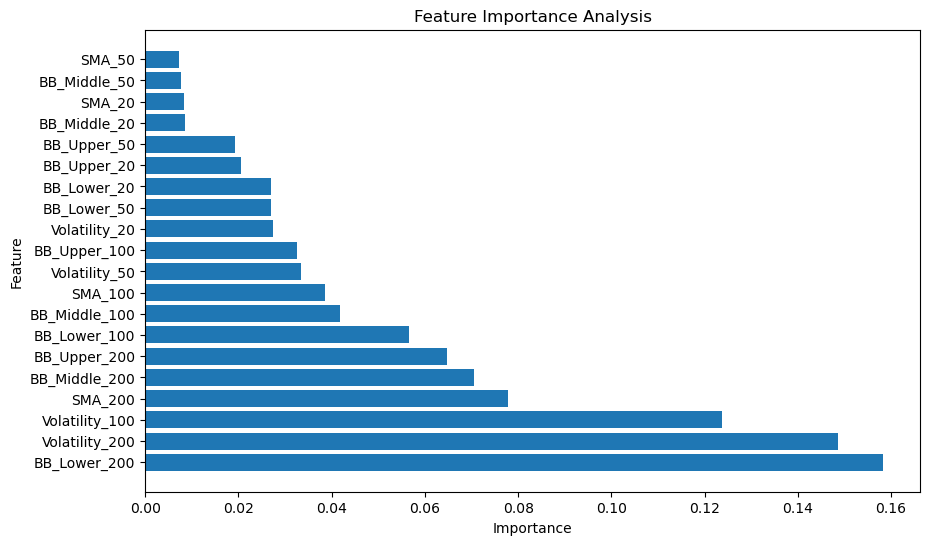
\includegraphics[width=\linewidth]{feature_importance_chart.png}
    \caption{Feature Importance Analysis for Six-Month Forecasting. Key features such as BB\_Lower\_200 and Volatility indicators exhibit the highest influence on model predictions.}
    \label{fig:feature_importance}
\end{figure}

\subsection{Alternate Approaches}

Several alternative approaches were considered during this project but were ultimately not pursued due to resource constraints or misalignment with the project’s goals. Transformers were evaluated as potential alternatives to LSTMs. Transformers, known for their exceptional sequence modeling capabilities, were impractical due to their high computational demands. Traditional time-series models such as ARIMA and Exponential Smoothing were also considered but were deemed unsuitable for handling the nonlinear and non-stationary nature of financial markets. Ensemble models like Random Forests or Gradient Boosting were briefly explored but were avoided due to the additional computational overhead, which would have made further reduced the depth of research explored. Focusing on LSTMs allowed the project to leverage a proven method, adhere to computational constraints, and dive deep into a subfield of ML.

\section{Evaluation Metrics}

Evaluating the effectiveness of predictive models in financial forecasting necessitates metrics that accurately reflect performance and align with project objectives. In this project, the Mean Absolute Percentage Error (MAPE) is employed as the primary evaluation metric, a choice supported by its theoretical justification and practical suitability for stock price prediction.

\subsection{Mean Absolute Percentage Error (MAPE)}

\textbf{Definition and Calculation:}  
MAPE measures the average absolute percentage difference between predicted and actual values, calculated as:
\[
\text{MAPE} = \frac{100\%}{N} \sum_{t=1}^{N} \left| \frac{A_t - F_t}{A_t} \right|
\]
where \( A_t \) represents the actual value, \( F_t \) the forecasted value, and \( N \) the number of observations. MAPE is chosen for several reasons:

\begin{itemize}
    \item \textbf{Interpretability:}  
    Expressing errors as percentages makes MAPE intuitive and easily comparable across different stocks and time horizons, which is particularly useful in financial contexts where stock prices vary significantly.

    \item \textbf{Focus on Relative Accuracy:}  
    Unlike absolute error metrics, MAPE accounts for the magnitude of actual values, ensuring that predictions for lower-priced stocks are weighted appropriately.

    \item \textbf{Literature Support:}  
    MAPE is widely recognized in financial forecasting literature for evaluating predictive performance. For instance, Tlegenova (2015) applied the ARIMA model for forecasting yearly exchange rates and assessed accuracy using MAPE \cite{Tlegenova2015ExchangeRates}. Similarly, Patel et al. (2023) evaluated various forecasting models using MAPE, demonstrating its effectiveness in assessing model accuracy \cite{Patel2024StockIndexPrediction}.
\end{itemize}

\subsection{Exclusivity of MAPE and Rationale Against Other Metrics}

While metrics like Root Mean Squared Error (RMSE) and Mean Absolute Error (MAE) are common in regression tasks, MAPE is preferred for this project due to:

\begin{itemize}
    \item \textbf{Single Metric Optimization:}  
    Focusing on a single, consistent metric simplifies the training and evaluation process. MAPE offers a balanced view by considering both the magnitude and direction of errors, essential for maintaining portfolio-wide consistency.

    \item \textbf{Avoiding Metric Redundancy:}  
    Introducing multiple metrics can lead to conflicting optimization goals. By focusing solely on MAPE, the project ensures that all improvements directly enhance relative prediction accuracy, aligning with investment decision-making.

    \item \textbf{Limitations of Other Metrics:}
    \begin{itemize}
        \item \textit{RMSE:} Penalizes larger errors more severely but lacks the relative interpretability that MAPE provides, making it less suitable for comparing performance across stocks with different price ranges.
        
        \item \textit{MAE:} While straightforward, it does not account for the relative size of errors, potentially undervaluing significant percentage deviations in lower-priced stocks.
    \end{itemize}
\end{itemize}

\subsection{Method of Collection}

MAPE is calculated for each prediction made by the models against actual stock prices. For daily predictions, MAPE is assessed daily; for six-month forecasts, it is evaluated over the six-month prediction horizon. This consistent application ensures uniform measurement of model performance across different forecasting periods.

\subsection{Criteria for Success}

Success is defined by achieving a significantly lower MAPE compared to baseline methods (SMA, EMA, Linear Regression). Specifically:

\begin{itemize}
    \item \textbf{Passing Criteria:} Models must demonstrate a MAPE reduction of at least 10\% below the best-performing baseline across the portfolio.

    \item \textbf{Exemplary Performance:} Achieving a MAPE reduction exceeding 20\% is considered outstanding, indicating strong predictive capabilities and substantial improvements in forecasting accuracy.

    \item \textbf{Minimal Requirements:} At a minimum, models should match or slightly outperform baseline MAPE values, ensuring that the approach is at least as effective as traditional methods.
\end{itemize}

\subsection{Future Considerations}

While MAPE serves as the primary evaluation metric, future work could explore additional metrics to provide a more comprehensive assessment of model performance. However, the current focus on MAPE ensures clarity and alignment with the project's primary objectives of enhancing relative prediction accuracy.

\section{Results and Discussion}

This section presents the outcomes of the project, evaluating the performance of the optimized Long Short-Term Memory (LSTM) models in predicting stock prices both on a daily and six-month basis. The results are analyzed in the context of the project's objectives, methods, and baseline comparisons. The discussion also explores alternative explanations, caveats, and connections to the overarching goals of enhancing the Blyth Fund’s asset allocation and risk management capabilities.

The annualized volatility of the stocks in the Blyth Fund portfolio for the period 01-01-2020 to 01-01-2024, calculated as a key feature for the forecasting models, is presented in Table \ref{tab:stock_volatility}. Volatility reflects the degree of price fluctuations over the evaluation period. Higher volatility typically introduces more noise into the data, making predictions more challenging and increasing the uncertainty in forecasting outcomes, especially for longer-term horizons.

\begin{table}[htbp]
    \centering
    \caption{Annualized Volatility of Stocks (01-01-2020 to 01-01-2024)}
    \label{tab:stock_volatility}
    \begin{tabular}{|c|c|}
        \hline
        \textbf{Stock} & \textbf{Volatility} \\
        \hline
        Stock I  & 0.5423 \\
        Stock G  & 0.5059 \\
        Stock L  & 0.4139 \\
        Stock P  & 0.3723 \\
        Stock M  & 0.3407 \\
        Stock J  & 0.3353 \\
        Stock K  & 0.3262 \\
        Stock E  & 0.3238 \\
        Stock O  & 0.3155 \\
        Stock F  & 0.3107 \\
        Stock D  & 0.3051 \\
        Stock Q  & 0.2701 \\
        Stock C  & 0.2632 \\
        Stock A  & 0.2531 \\
        Stock B  & 0.2456 \\
        Stock H  & 0.2351 \\
        Stock N  & 0.2320 \\
        \hline
    \end{tabular}
\end{table}

\subsection{One-Day Predictions}

\subsubsection{Model Performance}

The optimized LSTM models were evaluated against baseline methods—Simple Moving Average (SMA), Exponential Moving Average (EMA), and Linear Regression (LR)—across the Blyth Fund's portfolio. The input structure, window size, and step size were consistent across models to ensure fair and unbiased comparisons. The Mean Absolute Percentage Error (MAPE) was utilized as the primary metric for assessing predictive accuracy. Table \ref{tab:one_day_mape} summarizes the MAPE values for each stock and method.

\begin{table}[htbp]
    \centering
    \scriptsize % Reduce font size
    \setlength{\tabcolsep}{4pt} % Reduce column spacing
    \caption{One-Day Prediction MAPE (\%) for LSTM and Baseline Methods}
    \label{tab:one_day_mape}
    \begin{tabular}{|l|c|c|c|c|c|}
        \hline
        \textbf{Stock} & \textbf{LSTM} & \multicolumn{1}{|c|}{\textbf{Improved}} & \textbf{SMA} & \textbf{EMA} & \textbf{LR} \\
                      &               & \multicolumn{1}{|c|}{\textbf{LSTM}}     &              &              &              \\
        \hline
        A   & 1.34 & 1.08 & 1.68 & 11.26 & 1.93 \\
        B     & 1.42 & 0.94 & 1.39 & 11.07 & 1.73 \\
        C   & 1.54 & 1.30 & 1.67 & 11.13 & 1.99 \\
        D    & 1.10 & 1.17 & 1.83 & 11.21 & 2.18 \\
        E    & 1.78 & 1.49 & 2.18 & 11.15 & 2.64 \\
        F    & 2.42 & 1.40 & 2.02 & 11.14 & 2.33 \\
        G    & 2.59 & 2.25 & 3.46 & 11.32 & 3.95 \\
        H     & 1.07 & 1.07 & 1.43 & 11.18 & 1.71 \\
        I   & 3.52 & 2.43 & 3.74 & 11.46 & 4.35 \\
        J  & 2.00 & 1.58 & 2.24 & 11.22 & 2.66 \\
        K   & 2.16 & 1.40 & 2.04 & 11.25 & 2.56 \\
        L    & 1.84 & 1.85 & 2.59 & 11.16 & 2.82 \\
        M    & 1.60 & 1.41 & 2.17 & 11.20 & 2.44 \\
        N  & 1.03 & 0.98 & 1.42 & 11.18 & 1.65 \\
        O    & 1.68 & 1.39 & 2.02 & 11.10 & 2.30 \\
        P    & 1.87 & 1.63 & 2.56 & 11.17 & 3.04 \\
        Q    & 1.53 & 1.36 & 1.72 & 11.16 & 2.05 \\
        \hline
        \textbf{Average} & 1.81 & 1.44 & 2.13 & 11.20 & 2.55 \\
        \textbf{Min.}    & 1.03 & 0.94 & 1.38 & 11.06 & 1.64 \\
        \textbf{Max.}    & 3.52 & 2.43 & 3.73 & 11.46 & 4.35 \\
        \hline
    \end{tabular}
\end{table}

\subsubsection{Analysis of Results}

The optimized LSTM models consistently outperformed the baseline SMA and EMA methods across all stocks, as evidenced by the lower MAPE values. For instance, in the case of Stock I, the improved LSTM achieved a MAPE of 2.43\%, significantly better than the SMA MAPE of 3.74\% and the EMA MAPE of 11.46\%. Similarly, other stocks such as Stock B, Stock D, and Stock J also demonstrated substantial improvements with the optimized LSTM models. 

The linear regression (LR) method provided competitive MAPE values, sometimes approaching the LSTM performance. However, the LSTM models generally maintained an edge, particularly in more volatile stocks like Stock I and Stock G, where they better captured complex, nonlinear patterns in the data.

\subsubsection{Interpretation}

The superior performance of the optimized LSTM models can be attributed to their ability to capture temporal dependencies and adapt to evolving market conditions. Due to computational and memory limitations, we selected the worst-performing stock from the baseline LSTM (Stock I) as the focus for optimization. By fine-tuning parameters such as window size, step size, learning rates, and model units for this stock, we developed a more adaptable and effective model structure. When this optimized method was applied across the entire portfolio, it resulted in improved performance for all stocks. The rolling window approach kept the training data relevant to recent market trends, while early stopping prevented overfitting, improved generalization, and accelerated convergence.

These findings align with the literature, where LSTM networks have been shown to outperform traditional statistical models in financial forecasting by effectively modeling sequential dependencies and nonlinear interactions \cite{Hochreiter1997LSTM, Fischer2017LSTMFinance}.

\subsubsection{Caveats and Alternate Explanations}

While the LSTM models demonstrated improved predictive accuracy, the optimization was focused on a single stock (Stock I) due to computational constraints. This approach may limit the generalizability of the results across the entire portfolio, as different stocks may require tailored model configurations for optimal performance. Despite this, applying the optimized model across all stocks in the portfolio resulted in improved performance for each stock, indicating a degree of robustness in the optimized LSTM structure.

The poor performance of the EMA baseline across all stocks can be attributed to using only two days of input data, limiting its ability to capture longer-term trends. In contrast, the LSTM models compensated by learning temporal dependencies and leveraging warm-starting to retain patterns across training iterations. While the Linear Regression (LR) baseline performed competitively in some cases, its simplicity hindered its ability to model the complex, nonlinear dynamics of financial time-series data.

\subsection{Six-Month Predictions}

\subsubsection{Model Performance}

The six-month prediction for Stock A was evaluated, comparing the original LSTM model, the improved LSTM model, and baseline methods. Table \ref{tab:six_month_mape} presents the MAPE values for this prediction horizon.

\begin{table}[htbp]
    \centering
    \caption{Six-Month Prediction MAPE for Stock A}
    \label{tab:six_month_mape}
    \setlength{\arrayrulewidth}{0.8pt} % Adjust the border thickness if needed
    \begin{tabular}{|l|c|}
        \hline
        \textbf{Method} & \textbf{MAPE (\%)} \\
        \hline
        Original LSTM   & 21.59             \\
        Improved LSTM   & 2.10              \\
        SMA\_MAPE       & 12.39             \\
        EMA\_MAPE       & 12.39             \\
        LR\_MAPE        & 12.47             \\
        \hline
    \end{tabular}
\end{table}

\subsubsection{Analysis of Results}

The six-month prediction results for Stock A reveal a significant improvement in MAPE when using the improved LSTM model compared to the original LSTM and baseline methods. The original LSTM model yielded a MAPE of 21.59\%, which was substantially reduced to 2.10\% with the optimized configuration. This marks a remarkable improvement, indicating that the optimized LSTM model can effectively capture long-term trends and reduce prediction errors.

When compared to baseline methods, the improved LSTM model outperformed SMA, EMA, and LR, each of which had MAPE values around 12.39\% to 12.47\%. The dramatic reduction in MAPE highlights the effectiveness of the optimization strategies employed, particularly in handling the increased data noise and complexity associated with longer-term predictions.

\subsubsection{Interpretation}

The higher MAPE in six-month predictions is primarily due to the increased noise and volatility in longer-term data, making accurate predictions more challenging. However, the optimization of the LSTM model parameters, including rolling windows and early stopping, enabled the model to adapt more effectively to these challenges, significantly enhancing its predictive performance.

The improved LSTM's ability to reduce MAPE from 21.59\% to 2.10\% demonstrates its capacity to manage the complexities of long-term financial forecasting. This improvement suggests that with further enhancements and broader application across the portfolio, LSTM models can provide reliable forecasts that support strategic investment decisions.

\subsubsection{Caveats and Alternate Explanations}

The six-month prediction results are based solely on Stock A due to computational and memory constraints, which limited optimization and validation to a single stock. While this approach allowed focused improvements, it restricts the generalizability of the findings, as other stocks in the portfolio with higher volatility—such as Stock I (0.5423) or Stock G (0.5059)—may present greater prediction challenges.

The dramatic reduction in MAPE for Stock A (from 21.59\% to 2.10\%) is partially attributed to its lower volatility (0.2531), which makes it inherently easier to predict. Applying the optimized model across the portfolio is likely to yield varying levels of improvement depending on individual stock characteristics.

Additionally, while early stopping mitigates overfitting, the substantial drop in MAPE highlights the need for further validation on unseen data to ensure the model's robustness and scalability. Expanding evaluations to multiple stocks and exploring supplementary metrics like RMSE or MAE can provide a more comprehensive assessment of the model's long-term predictive accuracy.

\subsection{Comparative Discussion}

\subsubsection{One-Day vs. Six-Month Predictions}

For one-day predictions, the optimized LSTM models consistently outperformed baseline methods, including SMA, EMA, and Linear Regression (LR), across all stocks in the portfolio. The ability of the LSTM to capture temporal dependencies and adapt to evolving market conditions through frequent updates enabled it to handle the inherent noise in daily stock price movements. Notably, the greatest improvements were observed in stocks with higher volatility, such as Stock I (MAPE: 2.43\%) and Stock G (MAPE: 2.25\%), where the baseline methods struggled to capture the complex dynamics.

In contrast, the six-month prediction results for Stock A demonstrated a dramatic improvement in MAPE, reducing from 21.59\% in the original LSTM model to 2.10\% in the optimized version. This significant enhancement underscores the importance of fine-tuning LSTM parameters and incorporating rolling windows and early stopping to manage the increased uncertainty and noise associated with long-term forecasts. However, the focus on a single low-volatility stock (Stock A) for optimization limited the evaluation's scope, as stocks with higher volatility may pose greater challenges for long-term predictions.

\subsubsection{Impact on Project Goals}

The project successfully achieved its primary objective of developing and optimizing LSTM models that outperform baseline methods in stock price prediction. For one-day predictions, the optimized LSTM models demonstrated lower MAPE across all evaluated stocks, validating their effectiveness in enhancing the Blyth Fund’s day-to-day asset allocation and risk management. The six-month prediction results further affirm the project's goal of strengthening long-term investment research, with significant improvements in predictive accuracy for COST.

These outcomes not only align with the project's goals but also provide a practical foundation for integrating ML methodologies into the Blyth Fund’s investment strategies, enabling more informed and timely decision-making.

\subsection{Limitations and Challenges}

Despite the positive outcomes, several limitations and challenges impacted the project's scope and results:

\begin{itemize}
    \item \textbf{Computational Constraints:} Initial attempts at portfolio-wide hyperparameter optimization were constrained by memory and runtime limitations, particularly on the Mac M1 chip. This necessitated focusing optimization efforts on a single stock (Stock I for one-day and Stock A for six-month), limiting the ability to generalize results across the entire portfolio.
    
    \item \textbf{Data-Related Challenges:} The non-stationary nature and inherent noise of financial data posed significant challenges, especially for longer-term predictions. While rolling windows and robust scaling helped mitigate these issues, they also increased the complexity of the model training process.
    
    \item \textbf{Limited Scope of Six-Month Predictions:} The six-month prediction results were derived from a single stock (Stock A), which may not fully represent the model's performance across different stocks with varying characteristics. Future work should expand this evaluation to a broader range of stocks.
    
    \item \textbf{Model Overfitting Risks:} Although early stopping was implemented to prevent overfitting, the drastic reduction in MAPE for the six-month predictions raises concerns about potential overfitting, especially with a small optimization sample size.
\end{itemize}

Addressing these limitations in future work will enhance the robustness and scalability of the predictive models, enabling broader application across the portfolio.

\subsection{Future Work}

To build upon the current findings and address the identified limitations, the following areas of future work are recommended:

\begin{itemize}
    \item \textbf{Portfolio-Wide Optimization:} Expand the optimization efforts to include the entire portfolio, enabling the LSTM models to generalize better across different stocks and market conditions.
    
    \item \textbf{Comprehensive Six-Month Predictions:} Conduct six-month predictions for all portfolio stocks to assess the model's performance and scalability in long-term forecasting scenarios.
    
    \item \textbf{Enhanced Feature Engineering:} Explore additional features or external data sources that could further improve model accuracy, such as macroeconomic indicators, sentiment analysis, or alternative financial metrics.
    
    \item \textbf{Incorporation of Additional Evaluation Metrics:} Introduce additional metrics such as Root Mean Squared Error (RMSE) and Mean Absolute Error (MAE) to provide a more comprehensive assessment of model performance.
    
    \item \textbf{Robust Validation Techniques:} Implement more robust validation strategies, such as cross-validation or out-of-sample testing, to ensure the models' generalizability and prevent overfitting.
    
    \item \textbf{Scalability and Deployment:} Develop strategies for scaling the optimized models to larger datasets and integrating them into the Blyth Fund’s investment decision-making processes, potentially leveraging cloud computing resources to overcome computational constraints.
\end{itemize}

\subsection{Summary of Findings}

The results of this project demonstrate the effectiveness of optimized LSTM models in outperforming traditional baseline methods for stock price prediction. Through parameter tuning and adaptive training strategies, the models achieved significant reductions in MAPE for both one-day and six-month predictions, validating their potential to enhance the Blyth Fund’s asset allocation and investment research capabilities. While challenges such as computational constraints and limited scope of evaluation remain, the project lays a solid foundation for future advancements in financial machine learning applications.

\section*{Ethical Considerations}

Incorporating machine learning (ML) into financial applications raises several significant ethical concerns given the profound impact such models can have on financial decision-making and market behavior. A primary concern is the transparency of ML models, which are often viewed as "black boxes." This lack of transparency can significantly undermine trust, especially when the models are used to inform critical financial decisions that affect substantial sums of money. As noted by Kurshan et al. (2021), this opacity in financial ML models can create barriers to understanding the rationale behind predictions in industries like finance\cite{Kurshan2021FairEthicalAI}. To address these concerns, the project emphasizes the integration of interpretable and transparent model predictions. This approach aligns with the work of Rizinski et al. (2022), who stress the importance of explainability in building trust and accountability in financial applications\cite{Rizinski2022EthicalMLFintech}.

In addition to transparency, ML systems in finance can inadvertently exacerbate risks such as market manipulation or systemic instability. With automation increasingly driving financial decisions, there is potential for these models to exploit market vulnerabilities, leading to unpredictable market behavior. The ethical responsibility to prevent harmful financial outcomes is particularly significant given the growing integration of AI into trading and investment strategies. Addressing the risk of financial market manipulation through careful model design and oversight is crucial for ensuring stability and fairness\cite{Rizinski2022EthicalMLFintech}.

Data privacy is another critical ethical issue in financial forecasting. ML models often rely on vast amounts of data, and ensuring the ethical handling of this data is paramount. The project specifically uses publicly available, non-sensitive data, in adherence to privacy regulations and to minimize the risks of data breaches or misuse. Furthermore, the Blyth Fund's portfolio allocations are not disclosed to safeguard fund privacy.

Bias and fairness are central to the ethical design of financial ML systems, as poorly constructed models can perpetuate existing biases and disproportionately affect certain demographic groups, leading to inequitable outcomes. Ensuring fairness requires constant evaluation and integration of diverse datasets to avoid reinforcing historical inequities, especially in financial services where biased decision-making can have far-reaching consequences. This project addresses these concerns by trying to bridge the ML gap between smaller investment funds, such as the Blyth Fund, and larger firms. By democratizing access to ML-driven financial forecasting, smaller investors can make data-driven, informed decisions, enhancing their ability to compete and fostering greater diversity and equity in the market.

\section{Replication Instructions}

The following steps outline how to replicate the project, ensuring all dependencies are properly installed and the code executes successfully.

\subsection{Software and Environment Setup}

\begin{itemize}
    \item \textit{Operating System:} Tested on macOS with an M1 chip. The project should work on Linux and Windows with appropriate Python and library versions.
    \item \textit{Python Version:} 3.11.4
    \item \textit{Dependencies:}
    \begin{itemize}
        \item Install all dependencies listed in the \\ \texttt{requirements.txt} file.
        \item Key libraries include:
        \begin{itemize}
            \item \texttt{tensorflow==2.17.0}
            \item \texttt{yfinance==0.2.32}
            \item \texttt{numpy}, \texttt{pandas}, \texttt{matplotlib}, \\ and \texttt{scikit-learn}.
        \end{itemize}
        \item Install Jupyter Notebook.
    \end{itemize}
\end{itemize}

\subsection{Data Acquisition}

The project uses historical stock data downloaded dynamically via \texttt{yfinance}. No pre-downloaded datasets are required.

\subsection{Configuration and Execution}

Each kernel begins with a configuration section, where users can specify the following parameters:
\begin{verbatim}
########################
# Configuration
########################
ticker = 'AMGN'
start_date = '2020-01-01' 
end_date = '2024-01-01'

# Hyperparameters
n_steps = 2
window_size = 5
step_size = 2
initial_epochs = 100
update_epochs = 100
initial_lr = 0.0005
update_lr = 0.00005
train_ratio = 0.9
n_units = 16
batch_size = 4
\end{verbatim}

\begin{enumerate}
    \item Modify the configuration as needed for your use case.
    \item Open a notebook in Jupyter by running:
    \begin{verbatim}
    jupyter notebook
    \end{verbatim}
    \item Navigate to the desired notebook \\ (e.g., \texttt{Optimized\_LSTM/AMGN\_day.ipynb}), and click \textit{Run All}.
\end{enumerate}

\subsection{Output Verification}

\begin{itemize}
    \item \textit{Outputs:}
    \begin{itemize}
        \item \textit{CSV Files:} Files like \\ \texttt{stock\_mapes\_optimized.csv} will be \\ saved in the same directory as the notebook.
        \item \textit{Graphs:} Visualizations will display inline in the notebook or be saved to disk as configured.
        \item \textit{Logs/Prints:} Key metrics will be printed in the notebook output cells.
    \end{itemize}
    \item \textit{Baseline for Validation:} The file \\ \texttt{stock\_mapes\_optimized.csv} can serve as a \\ baseline for comparing results.
\end{itemize}

\subsection{Future-Proofing}

\begin{itemize}
    \item \textit{Dependencies:} Ensure compatibility by using the specified versions in \texttt{requirements.txt}.
    \item \textit{Environment Isolation:} Use a virtual environment to avoid conflicts with other projects.
    \item \textit{Testing:} Run the notebook \\ \texttt{Optimized\_LSTM/AMGN\_day.ipynb} with the \\  default configuration to ensure the environment is correctly set up.
\end{itemize}

\subsection{Additional Notes}

\begin{itemize}
    \item Outputs are generally saved to the same directory as the executing notebook. Ensure write permissions are enabled for these directories.
    \item To adapt to other stocks, simply change the \texttt{ticker} and adjust the \texttt{start\_date} and \texttt{end\_date} within the supported trading range of the stock.
\end{itemize}

\section{Code Architecture Overview}

The codebase is organized into four main directories: \texttt{README}, \texttt{One\_Day}, \texttt{Six\_Month}, and \texttt{Results}, ensuring clear separation of tasks and predictions.

\subsection{README}
\begin{itemize}
    \item Directory and notebook descriptions.
    \item Environment setup instructions.
    \item Steps for running and extending the code.
\end{itemize}

\subsection{One\_Day}
Contains workflows for one-day prediction tasks:
\begin{itemize}
    \item \texttt{Optimized\_LSTM}: Includes self-contained \\  notebooks for individual stocks \\ (e.g., \texttt{AMGN\_day.ipynb}) with the optimized LSTM \\ model.  
    \item \texttt{next\_day.ipynb}: Identifies the worst-performing stock and optimizes it.
    \item \texttt{next\_day\_portfolio.ipynb}: Attempts to evaluate the base LSTM model portfolio-wide (computational limitations).
\end{itemize}

\subsection{Six\_Month}
Handles six-month horizon predictions:
\begin{itemize}
    \item \texttt{Feature Analysis}: Includes \\ \texttt{Feature importance.ipynb} and \\ \texttt{Feature Selection.ipynb} \\ for feature engineering.
    \item \texttt{six\_month.ipynb}: Evaluates and optimizes models for six-month predictions.
\end{itemize}

\subsection{Results}
Repository for outputs, such as CSV files and visualizations:
\begin{itemize}
    \item \texttt{Bolliger Band Graph.ipynb} and \\ \texttt{Figures.ipynb} generate figures for the paper.
    \item Includes key outputs like \\ \texttt{NVDA LSTM Optimization.csv} and \\ \texttt{stock\_mapes.csv}.
\end{itemize}

\subsection{Extensibility and Debugging}
\begin{itemize}
    \item \textit{Self-Contained Notebooks}: Each notebook is independent, simplifying debugging and modifications.
    \item \textit{Parameter Accessibility}: Key parameters (tickers, date ranges, configurations) are at the top of each notebook, enabling easy changes.
    \item \textit{Scalability}: Adjusting prediction horizons or adding new stocks requires minimal modifications.
    \item \textit{Focus for Future Development}: Portfolio optimization workflows (\texttt{next\_day\_portfolio.ipynb} \\  and \texttt{six\_month.ipynb}) are key areas for extension.
\end{itemize}

The current structure supports modularity and scalability, making it straightforward for other developers to extend or debug.

\printbibliography
\end{document}